\documentclass{article}
\usepackage[utf8]{inputenc}

\title{Core RL Behavior Suite Report}

\usepackage{natbib}
\usepackage{graphicx}
\usepackage{url}

\newcommand{\fullname}{Core RL Behavior Suite}
\newcommand{\shortname}{\texttt{bsuite}}
\newcommand{\github}{\url{github.com/deepmind/bsuite}}
\newcommand{\fullreport}{\url{ADD-LINK-HERE}}

\begin{document}

\vspace*{-100pt}
{\let\newpage\relax\maketitle}

\vspace*{20pt}

The \fullname  (in short \shortname)  is a collection of carefully-designed
experiments that investigate core capabilities of a reinforcement learning (RL)
agent by collecting clear, informative and scalable problems that capture key
issues in the design of learning algorithms. The environment and experiment code
can be found at \github, and automates evaluation and analysis of any agent on
\shortname. Below you can observe how the algorithms we considered compare
across various dimensions of learning.

\begin{figure}[h!]
\centering
\vspace*{20pt}
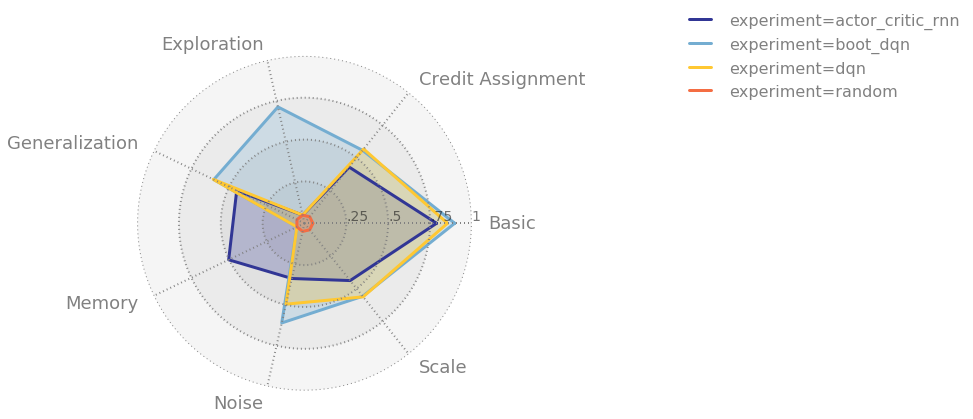
\includegraphics[width=0.9\linewidth]{images/radar_plot.png}
\caption{Summary analysis: The dimensions considered are 1. basic RL,
2. credit assignment, 3. exploration, 4. generalization, 5. memory,
6. robustness to noise, 7. robustness to scaling issues. On each of these
dimensions the score of a random agent is 0, and maximum performance is 1.}
\label{fig:universe}
\vspace*{20pt}
\end{figure}

\noindent The score reported for each of these dimensions summarizes a number
of experiments evaluating the algorithm's performance and its scalability with
the relevant difficulty knobs. A detailed analysis of each of these experiments
may be found in a notebook hosted on Colaboratory: \fullreport.

\end{document}
